\section{Introduction}

While deep learning systems have achieved great performance when sufficient amounts of labeled data are available~\cite{Lecun2015, HeZRS16, ShelhamerLD17},
there has been growing interest in reducing the required amount of data.
%
Few-shot learning tasks have been defined for this purpose. 
%
The aim is to learn new concepts from few labeled examples, e.g. 1-shot learning~\cite{FeiFeiFP06}.
%
While humans tend to be highly effective in this context, often grasping the essential connection between new concepts and their own knowledge and experience, it remains challenging for machine learning approaches.
E.g., on the CIFAR-100 dataset, a state-of-the-art method~\cite{OreshkinNIPS18} achieves only $40.1\%$ accuracy for 1-shot learning, compared to $75.7\%$ for the all-class fully supervised case~\cite{ClevertUH15}. 



\begin{figure}[t]
  \centering
  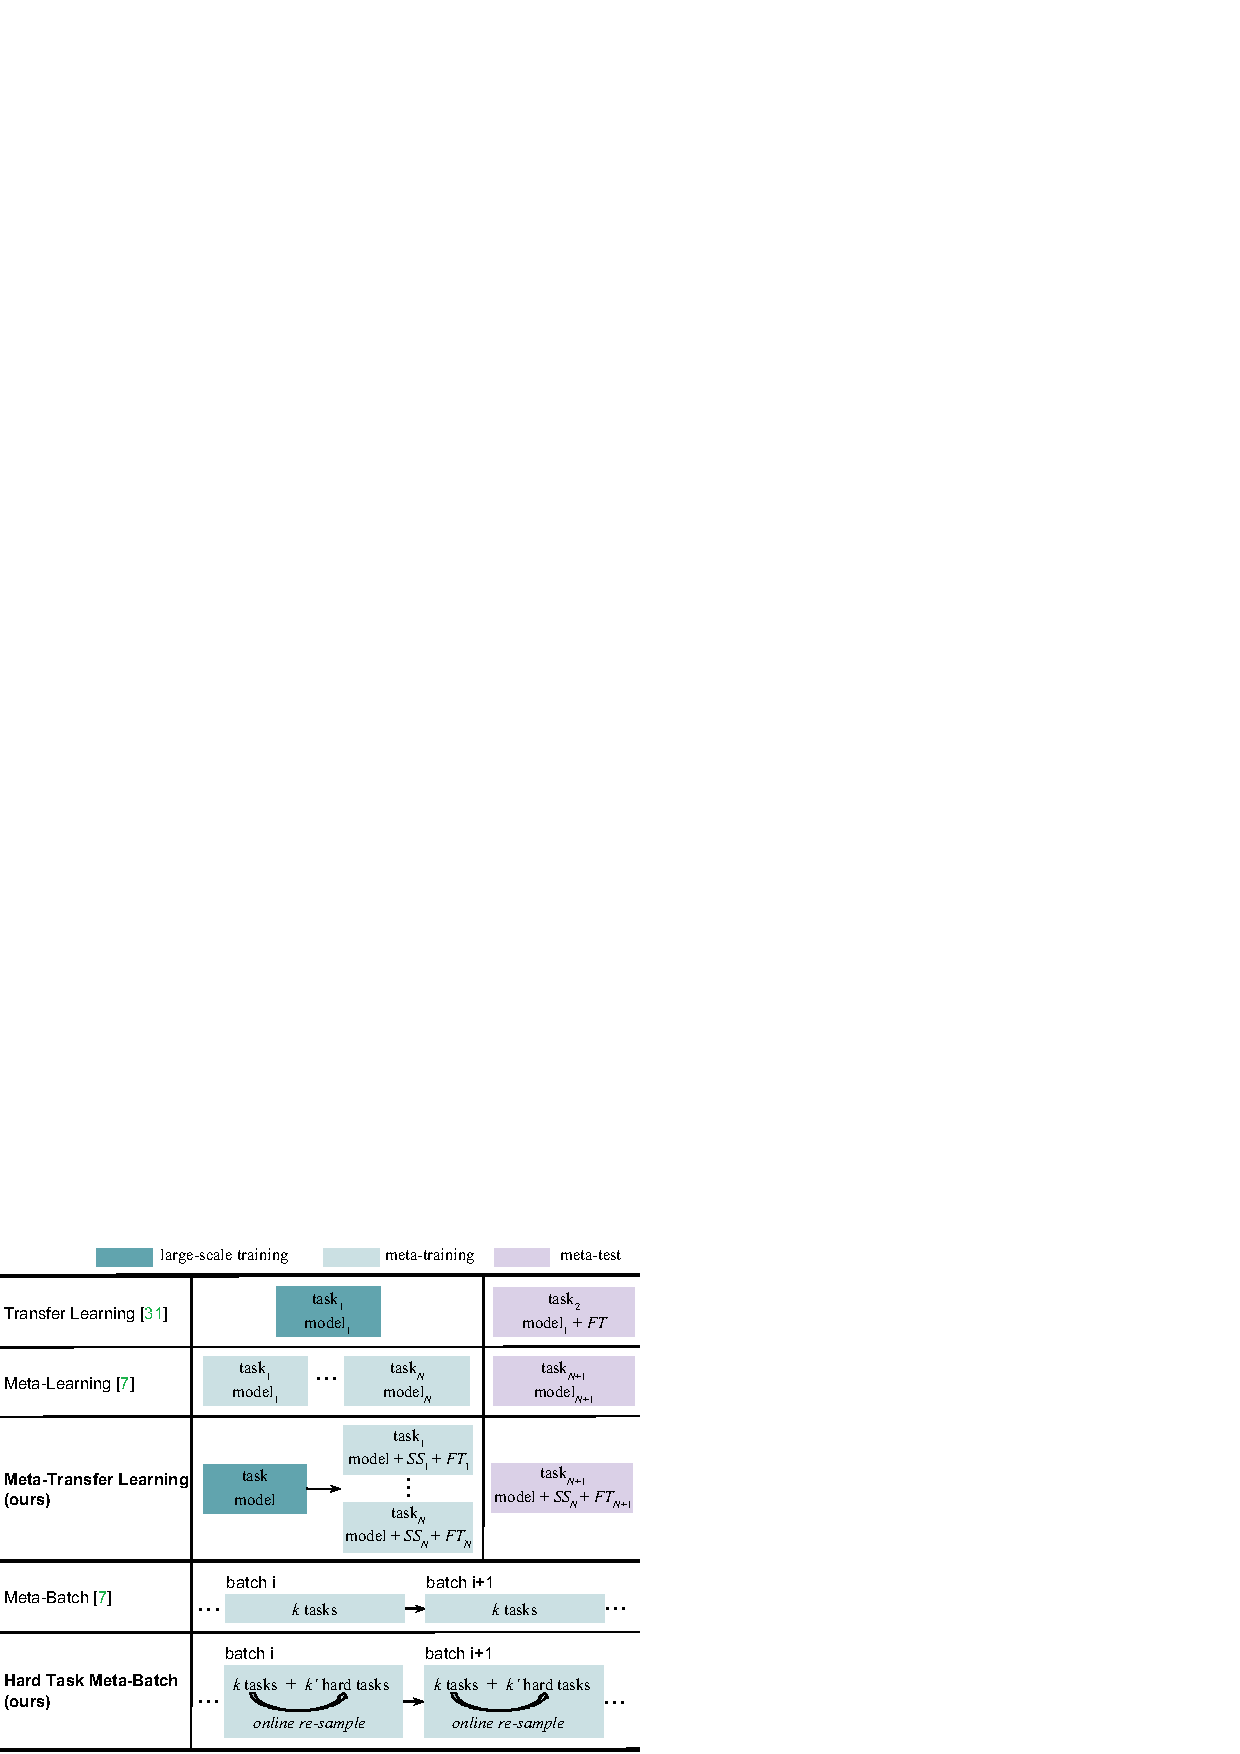
\includegraphics[width=0.99\linewidth]{figures/main_framework_tisser.pdf}
     \caption{Meta-transfer learning (MTL) is our meta-learning paradigm and hard task (HT) meta-batch is our training strategy. The upper three rows show the differences between MTL and related methods, transfer-learning~\cite{PanTKY11} and meta-learning~\cite{FinnAL17}.
     The bottom rows compare HT meta-batch with the conventional meta-batch~\cite{FinnAL17}. \emph{FT} stands for fine-tuning a classifier. \emph{SS} represents the \emph{Scaling} and \emph{Shifting} operations in our MTL method.}
  \label{main_framework_tisser}
  \vspace{-0.3cm}
\end{figure}

Few-shot learning methods can be roughly categorized into two classes: data augmentation and task-based meta-learning.
%
Data augmentation is a classic technique to increase the amount of available data and thus also useful for few-shot learning~\cite{KhorevaBIBS17}.
Several methods propose to learn a data generator e.g. conditioned on Gaussian noise~\cite{Mehrotra2017, SchwartzNIPS18, WangCVPR2018}. 
However, the generation models often underperform when trained on few-shot data~\cite{BartunovV18}.
%
An alternative is to merge data from multiple tasks which, however, is not effective due to variances of the data across tasks~\cite{WangCVPR2018}.
%

In contrast to data-augmentation methods, meta-learning is a task-level learning method~\cite{Bengio92, Naik92, Thrun1998}.
Meta-learning aims to accumulate experience from learning multiple tasks \cite{FinnAL17, RaviICLR2017, SnellSZ17, MunkhdalaiICML2017, GrantICLR2018}, while base-learning focuses on modeling the data distribution of a single task. 
A state-of-the-art representative of this, namely 
Model-Agnostic Meta-Learning (MAML), learns to search for the optimal initialization state to fast adapt a base-learner to a new task~\cite{FinnAL17}.
%
Its task-agnostic property makes it possible to generalize to few-shot supervised learning as well as unsupervised reinforcement learning~\cite{GrantICLR2018, FinnNIPS2018}.
%
However, in our view, there are two main limitations of this type of approaches limiting their effectiveness: i)~these methods usually require a large number of similar tasks for meta-training which is costly; and ii)~each task is typically modeled by a low-complexity base learner (such as a shallow neural network) to avoid model overfitting, thus being unable to use deeper and more powerful architectures. 
%
%
For example, for the miniImageNet dataset~\cite{VinyalsBLKW16}, MAML uses a \emph{shallow} CNN with only $4$ CONV layers and its optimal performance was obtained learning on $240k$ tasks.


In this paper, we propose a novel meta-learning method called \textbf{meta-transfer learning (MTL)} leveraging the advantages of both transfer and meta learning (see conceptual comparison of related methods in Figure~\ref{main_framework_tisser}). 
%
In a nutshell, MTL is a novel learning method that helps deep neural nets converge faster while reducing the probability to  overfit when using few labeled training data only.  
%
In particular, ``transfer'' means that DNN weights trained on large-scale data can be used in other tasks by two light-weight neuron operations: \emph{Scaling} and \emph{Shifting} (\emph{SS}), i.e. $\alpha X+\beta$. ``Meta'' means that the parameters of these operations can be viewed as hyper-parameters trained on few-shot learning tasks~\cite{MunkhdalaiICML2017, LiICML2018}.
%
%
Large-scale trained DNN weights offer a good initialization, enabling fast convergence of meta-transfer learning with fewer tasks, e.g. only $8k$ tasks for miniImageNet~\cite{VinyalsBLKW16}, $30$ times fewer than MAML~\cite{FinnAL17}.
%
Light-weight operations on DNN neurons have less parameters to learn, e.g. less than $\tfrac{2}{49}$ if considering neurons of size $7\times 7$ ($\tfrac{1}{49}$ for $\alpha$ and $<\tfrac{1}{49}$ for $\beta$), reducing the chance of overfitting.
%
In addition, these operations keep those trained DNN weights unchanged, and thus avoid the problem of ``catastrophic forgetting'' which means forgetting general patterns when adapting to a specific task~\cite{LopezPazNIPS17, McCloskey1989}.

%
%

The second main contribution of this paper is an effective meta-training curriculum.
Curriculum learning~\cite{BengioLCW09} and hard negative mining~\cite{ShrivastavaGG16} both suggest that faster convergence and stronger performance can be achieved by a better arrangement of training data.
%
%
Inspired by these ideas, we design our \textbf{hard task (HT) meta-batch} strategy to offer a challenging but effective learning curriculum.
%
As shown in the bottom rows of Figure~\ref{main_framework_tisser}, a conventional meta-batch contains a number of random tasks~\cite{FinnAL17}, but our HT meta-batch online re-samples harder ones according to past failure tasks with lowest validation accuracy.
%

Our overall contribution is thus three-fold:
i)~we propose a novel \textbf{MTL} method that learns to transfer large-scale pre-trained DNN weights for solving few-shot learning tasks; 
ii)~we propose a novel \textbf{HT meta-batch} learning strategy that forces meta-transfer to ``grow faster and stronger through hardship''; and 
iii)~we conduct extensive experiments on two few-shot learning benchmarks, namely miniImageNet~\cite{VinyalsBLKW16} and Fewshot-CIFAR100 (FC100)~\cite{OreshkinNIPS18}, and achieve the state-of-the-art performance. 
